% !TEX root = ../main.tex
% !TEX spellcheck = en_GB

\chapter{Analysis}
This section describes the analysis of the system; how the system is envisioned to be created, which subsystems it will consist of and the tasks each subsystem has to be able to perform to meet the specified requirements.

To fulfil the specified requirements in \nameref{chap:requirements} a module to locate the system, save the location and send the location must be present. Additionally a controller is needed to facilitate communication between the modules. This system interfaces with a server as shown in \cref{fig:BDD:unspecified}

\begin{figure}[H]
	\centering
	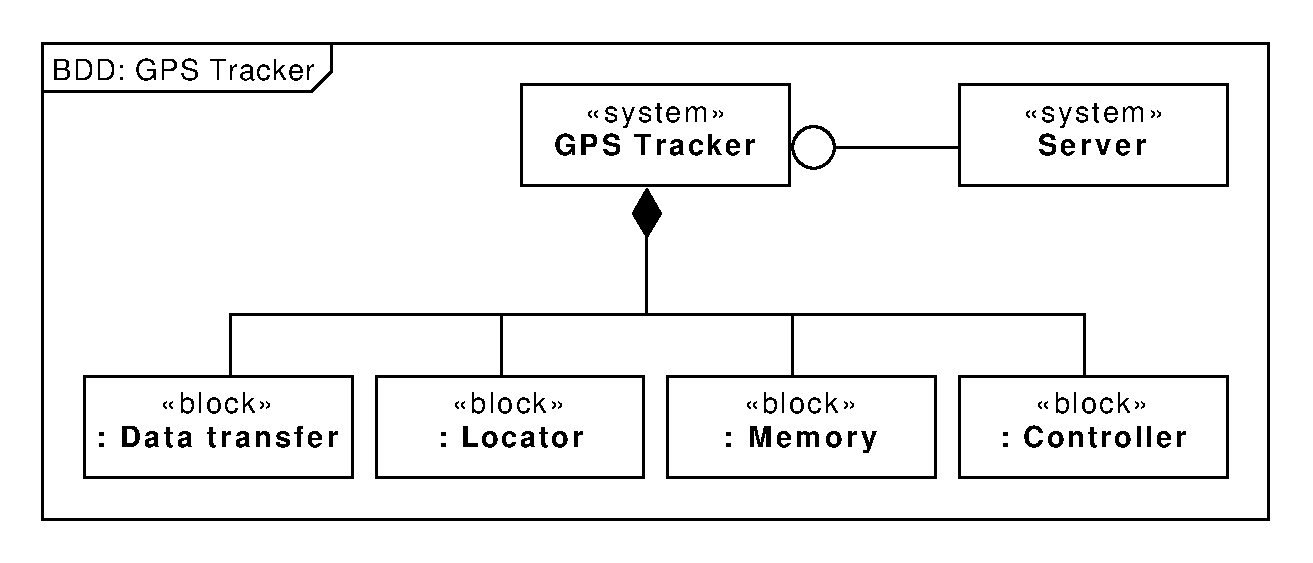
\includegraphics[width=0.7\linewidth]{gfx/Design/BDD_Unspecified.pdf}
	\caption{A high level BDD showing the parts of the \systemName, and the interface with a server.}
	\label{fig:BDD:unspecified}
\end{figure}

\FloatBarrier
